\documentclass[conference]{IEEEtran}
\IEEEoverridecommandlockouts
% The preceding line is only needed to identify funding in the first footnote. If that is unneeded, please comment it out.
\usepackage{cite}
\usepackage{amsmath,amssymb,amsfonts}
\usepackage{algorithmic}
\usepackage{graphicx}
\usepackage{textcomp}
\usepackage{xcolor}
\usepackage{lipsum}

\def\BibTeX{{\rm B\kern-.05em{\sc i\kern-.025em b}\kern-.08em
    T\kern-.1667em\lower.7ex\hbox{E}\kern-.125emX}}
\begin{document}

\title{Conference Paper Title*\\
    % \thanks{Identify applicable funding agency here. If none, delete this.}
}

\author{\IEEEauthorblockN{1\textsuperscript{st} Given Name Surname}
    \IEEEauthorblockA{\textit{dept. name of organization (of Aff.)} \\
        \textit{name of organization (of Aff.)}\\
        City, Country \\
        email address or ORCID}
    \and
    \IEEEauthorblockN{2\textsuperscript{nd} Given Name Surname}
    \IEEEauthorblockA{\textit{dept. name of organization (of Aff.)} \\
        \textit{name of organization (of Aff.)}\\
        City, Country \\
        email address or ORCID}
    \and
    \IEEEauthorblockN{3\textsuperscript{rd} Given Name Surname}
    \IEEEauthorblockA{\textit{dept. name of organization (of Aff.)} \\
        \textit{name of organization (of Aff.)}\\
        City, Country \\
        email address or ORCID}
}

\maketitle

\begin{abstract}
    This document is a model and instructions for \LaTeX.
    This and the IEEEtran.cls file define the components of your paper [title, text, heads, etc.]. *CRITICAL: Do Not Use Symbols, Special Characters, Footnotes,
    or Math in Paper Title or Abstract.
\end{abstract}

\begin{IEEEkeywords}
    component, formatting, style, styling, insert
\end{IEEEkeywords}

\section{Introduction}
\lipsum[1]

\section{New Section A}

\subsection{My subsection A}
\lipsum[1]

\section{Prepare Your Paper Before Styling}
\lipsum[1-2]

\subsection{Abbreviations and Acronyms}\label{AA}
\lipsum[1]

\subsection{Units subsection}
\begin{itemize}
    \item \lipsum[1]
    \item \lipsum[1]
    \item \lipsum[1]
    \item \lipsum[1]
\end{itemize}

\subsection{Equations subsection}
Number equations consecutively. To make your
equations more compact, you may use the solidus (~/~), the exp function, or
appropriate exponents. Italicize Roman symbols for quantities and variables,
but not Greek symbols. Use a long dash rather than a hyphen for a minus
sign. Punctuate equations with commas or periods when they are part of a
sentence, as in:
\begin{equation}
    a+b=\gamma\label{eq_ab}
\end{equation}

Be sure that the
symbols in your equation have been defined before or immediately following
the equation. Use ``\eqref{eq_ab}'', not ``Eq.~\eqref{eq_ab}'' or ``equation \eqref{eq_ab}'', except at
the beginning of a sentence: ``Equation \eqref{eq_ab} is . . .''

\subsection{subsection about BibTeX}
\underline{{\BibTeX} does not work by magic.} \textit{It doesn't get the bibliographic
data from thin air but from .bib files.} \textbf{If you use {\BibTeX} to produce a
bibliography you must send the .bib files.}

\subsection{Some Common Mistakes subsection}\label{SCM}
\begin{itemize}
    \item example items
    \item example items
    \item example items
    \item example items
    \item example items
    \item example items
    \item example items
    \item example items
    \item example items
    \item There is no period after the ``et'' in the Latin abbreviation ``et al.''.
    \item The abbreviation ``i.e.'' means ``that is'', and the abbreviation ``e.g.'' means ``for example''.
\end{itemize}
An excellent style manual for science writers is \cite{b7}.

\subsection{Another subsection}
\lipsum[1]

\subsection{Identify the Headings}
\lipsum[1-2]

\subsection{Figures and Tables}
\paragraph{Positioning Figures and Tables} Use the abbreviation
``Fig.~\ref{figx}'', even at the beginning of a sentence.

\begin{table}[htbp]
    \caption{Table Type Styles}
    \begin{center}
        \begin{tabular}{|c|c|c|c|}
            \hline
            \textbf{Table} & \multicolumn{3}{|c|}{\textbf{Column Head}}         \\
            \cline{2-4}
            \textbf{Head}  & column subhead & b & a \\
            \hline
            copy           & More table copy$^{\mathrm{a}}$ & b & a \\
            \hline
            \multicolumn{4}{l}{$^{\mathrm{a}}$Sample of a Table footnote.}
        \end{tabular}
        \label{tabx}
    \end{center}
\end{table}

\begin{figure}[htbp]
    \centerline{
\includegraphics[width=0.25\textwidth]{images/gato.png}}
    \caption{Example of a figure caption.}
    \label{figx}
\end{figure}

\paragraph{Another paragraph} Use the abbreviation
``Fig.~\ref{figy}'', even at the beginning of a sentence.
\begin{figure}[htbp]
    \centerline{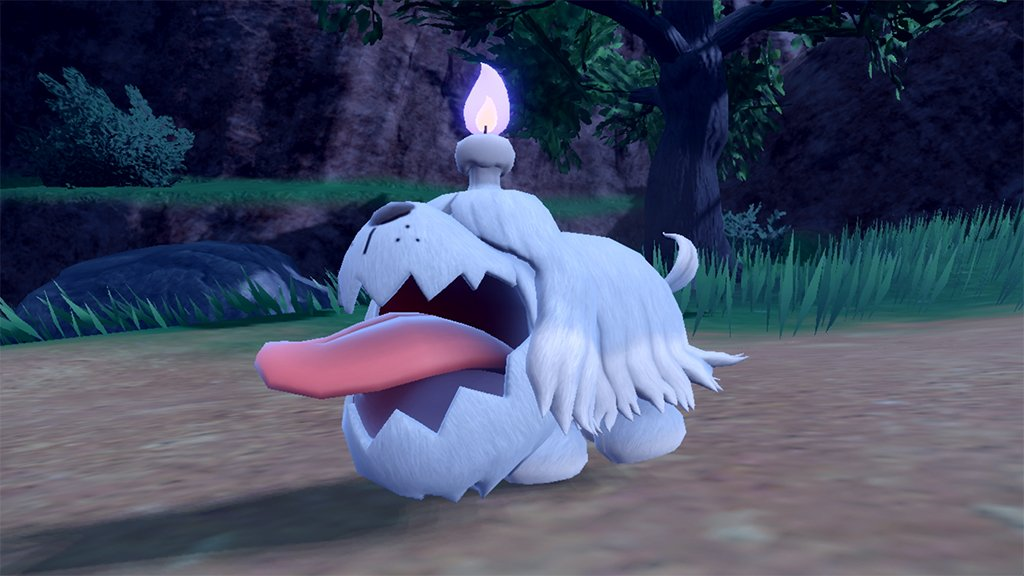
\includegraphics[width=0.25\textwidth]{images/perro.jpg}}
    \caption{Example of a figure caption.}
    \label{figy}
\end{figure}

\paragraph{Another paragraph} Use the abbreviation
``Fig.~\ref{figz}'', even at the beginning of a sentence.
\begin{figure}[htbp]
    \centerline{
\includegraphics[width=0.25\textwidth]{images/raton.jpg}}
    \caption{Example of a figure caption.}
    \label{figz}
\end{figure}

\section*{Acknowledgment section}
some text of example

\section*{References section}

Please number citations consecutively within brackets \cite{b2}. The
sentence punctuation follows the bracket \cite{b1}. Refer simply to the reference
number, as in \cite{b3}---do not use ``Ref. \cite{b3}'' or ``reference \cite{b3}'' except at
the beginning of a sentence: ``Reference \cite{b3} was the first $\ldots$''

Unless there are six authors or more give all authors' names; do not use
``et al.''. Papers that have not been published, even if they have been
submitted for publication, should be cited as ``unpublished'' \cite{b4}. Papers
that have been accepted for publication should be cited as ``in press'' \cite{b5}.
Capitalize only the first word in a paper title, except for proper nouns and
element symbols.For papers published in translation journals, please give the English
citation first, followed by the original foreign-language citation \cite{b6}.

\bibliographystyle{IEEEtran}
\bibliography{references}
% \begin{thebibliography}{00}
%     \bibitem{b1} G. Eason, B. Noble, and I. N. Sneddon, ``On certain integrals of Lipschitz-Hankel type involving products of Bessel functions,'' Phil. Trans. Roy. Soc. London, vol. A247, pp. 529--551, April 1955.
%     \bibitem{b2} J. Clerk Maxwell, A Treatise on Electricity and Magnetism, 3rd ed., vol. 2. Oxford: Clarendon, 1892, pp.68--73.
%     \bibitem{b3} I. S. Jacobs and C. P. Bean, ``Fine particles, thin films and exchange anisotropy,'' in Magnetism, vol. III, G. T. Rado and H. Suhl, Eds. New York: Academic, 1963, pp. 271--350.
%     \bibitem{b4} K. Elissa, ``Title of paper if known,'' unpublished.
%     \bibitem{b5} R. Nicole, ``Title of paper with only first word capitalized,'' J. Name Stand. Abbrev., in press.
%     \bibitem{b6} Y. Yorozu, M. Hirano, K. Oka, and Y. Tagawa, ``Electron spectroscopy studies on magneto-optical media and plastic substrate interface,'' IEEE Transl. J. Magn. Japan, vol. 2, pp. 740--741, August 1987 [Digests 9th Annual Conf. Magnetics Japan, p. 301, 1982].
%     \bibitem{b7} M. Young, The Technical Writer's Handbook. Mill Valley, CA: University Science, 1989.
% \end{thebibliography}
\vspace{12pt}
\textcolor{red}{IEEE conference templates contain guidance text for composing and formatting 
conference papers. Please ensure that all template text is removed from your 
conference paper prior to submission to the conference. Failure to remove the 
template text from your paper may result in your paper not being published.}

end of my text
\end{document}
